L'analyse sémantique du Stibbons est effectué dans les classes Interpreter. Plus exactement dans 3 classes. Voir l'UML~\ref{interpreterUML} correspondant page~\pageref{interpreterUML}.

\begin{figure}[h]
\caption{\label{interpreterUML} UML de l'analyseur sémantique}
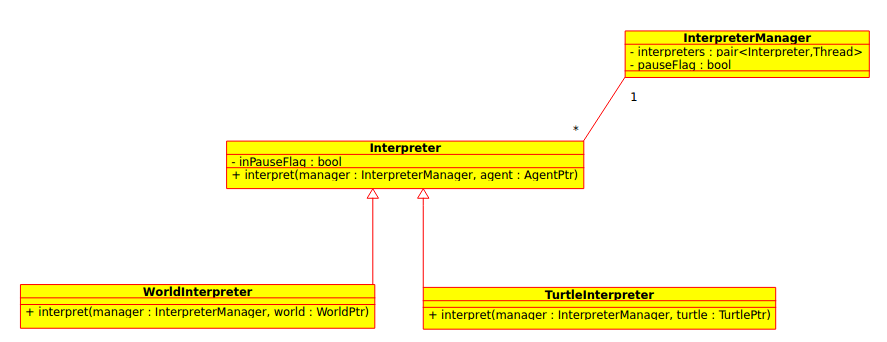
\includegraphics[scale=0.5]{doc/report/uml/interpreterUML.png}
\end{figure}

On a donc les classes \verb|TurtleInterpreter| et \verb|WorldInterpreter| qui héritent de la classe \verb|Interpreter|. Cette dernière analyse et provoque, dans le modèle, les actions liées au code stibbons écrit. Elle permet de gérer tout type d'interaction, du moment que ces actions ne sont pas liées à un monde ou une tortue. La classe \verb|TurtleInterpreter|, gère justement ce dernier type d'actions : celles liées à une tortue. Contrairement à \verb|WorldInterpreter| qui gère les actions du monde.

L'utilité de la classe \verb|InterpreterManager| est expliqué de manière détaillée dans la section \ref{remaniementInterpreter} (page~\pageref{remaniementInterpreter}).

Ainsi, pour avoir un exemple concret, si on demande à une tortue d'avancer en stibbons (ex : \verb|fd 10|), alors c'est le \verb|TurtleInterpreter| qui gèrera cette action.
A contrario, si on effectue une définition de fonction (ex : \verb|a = 10|) alors l'\verb|Interpreter| affectera la valeur \verb|10| à la propriété \verb|a| de l'agent courant.
Pour ce qui est du WorldInterpreter, il n'y a pas encore d'exemple possible, tout simplement car pour l'instant il n'y a pas d'actions spéciales pour le monde.

\subsection{Fonctionnalités}

\subsubsection{Sprint 1 \& 2}
Les deux premiers sprints ont été assez conséquent au niveau du nombre de fonctionnalités ajoutées.
En effet lors du sprint 1 on pouvait déjà effectuer les opérations de bases sur une tortue, telles que avancer, tourner, écrire, etc. De plus les opérations de calculs ainsi que la gestions de nombre ont été fait. En effet, il était nécessaire de gérer les nombres de manière à pouvoir indiquer à la tortue de quelle distance elle devait avancer.

Lors du deuxième sprint sont apparu les conditionnelles, ainsi que les boucles, les comparaisons binaires, les booléens et autres type (color, string, etc.), la création de nouveaux agents dans le code et les fonctions sans paramètres. Ce sprint fut alors une version déjà bien avancé de notre programme final.


\subsubsection{Sprint 3 à 5}
Les sprints suivants ont été plus léger. Non pas parce qu'il y avait moins de travail, car la gestion de l'interpréteur fut remanier à ce moment là, mais car il y avait moins de fonctionnalités à ajouter. En effet à partir du sprint 3, les fonctionnalités suivantes ont été rajoutés~:
\begin{itemize}
\item accès à la parenté et aux zones (en lecture seulement)~;
\item ajout des tables et de boucles dédiés (\verb|foreach|)~;
\item gestion de la vitesse et de la pause~;
\item ajout des communications avec le \verb|send| et le \verb|recv|.
\end{itemize}


\subsection{Remaniement de l'analyseur sémantique}
\label{remaniementInterpreter}

L'analyseur sémantique a d'abord été une seule classe~: la classe \verb|Interpreter|.
Cette dernière implémentait tout types d'actions a effectué pour n'importe quel type d'agent.
Cependant, lors de l'arrivée de la fonctionnalité d'ajout d'un nouvel agent (\verb|new agent|), nous nous sommes aperçu qu'il serait mieux d'avoir un interpréteur par type d'agent, ou plus précisement un interpréteur pour le monde, un pour les tortues et un pour les actions communes aux deux types.
Nous avons alors crée les deux classes~: \verb|WorldInterpreter| et \verb|TurtleInterpreter|.

De manière parallèle, la création du monde s'effectuait dans l'\verb|Interpreter|, puis dans le \verb|WorldInterpreter|, il fut alors nécessaire de crée une classe qui gérerait à la fois la création du monde et tout ce qui concernait l'application (la pause, le temps, les interpreteurs eux-mêmes). Nous avons alors décidé de crée la classe \verb|InterpreterManager|.
Cette classe connait ainsi tout les interpréteurs, permet de les prévenir d'une éventuelle pause du programme, de stocker les threads correspondants à chaque interpréteur, de crée un monde avec les pré-directives choisies~; c'est une sorte de gestionnaire d'interpréteurs.
